\documentclass[10pt]{article}

\usepackage[margin=0.8in]{geometry}
\usepackage{booktabs}
\usepackage{graphicx}
\usepackage{xcolor}
\usepackage{hyperref}
\usepackage{enumitem}
\usepackage{array}
\usepackage{tikz}
\usepackage[most]{tcolorbox}
\usetikzlibrary{arrows.meta, positioning}

\definecolor{riskred}{HTML}{B91C1C}
\definecolor{riskorange}{HTML}{C2410C}
\definecolor{riskyellow}{HTML}{A16207}
\definecolor{softred}{HTML}{FEF2F2}
\definecolor{softorange}{HTML}{FFF7ED}
\definecolor{softyellow}{HTML}{FEFCE8}
\definecolor{softblue}{HTML}{EFF6FF}
\definecolor{ink}{HTML}{111827}

\hypersetup{
  colorlinks=true,
  linkcolor=blue,
  urlcolor=blue
}

\newtcolorbox{findingbox}{
  colback=softred,
  colframe=riskred,
  arc=2mm,
  boxrule=0.9pt,
  left=6pt,
  right=6pt,
  top=6pt,
  bottom=6pt
}

\newtcolorbox{promptbox}[1]{
  title={#1},
  colback=softblue,
  colframe=blue!55!black,
  arc=2mm,
  boxrule=0.7pt,
  fonttitle=\bfseries,
  left=6pt,
  right=6pt,
  top=5pt,
  bottom=5pt
}

\title{\vspace{-1.2cm}FiDeLiS Internal Prompt Map}
\author{}
\date{}

\begin{document}
\maketitle
\vspace{-1.0cm}

\section*{Executive Finding}

\begin{findingbox}
The current FiDeLiS pipeline is not strictly KG-faithful at the final answer step.
For WebQSP, CWQ, and CR-LT, the final answer prompt allows the model to answer based on the retrieved reasoning path \emph{and your knowledge}.
This makes it possible for correct answers to come from the LLM's pretrained parametric knowledge rather than from the retrieved KG path.
\end{findingbox}

\section*{Pipeline View}

\begin{center}
\resizebox{\linewidth}{!}{%
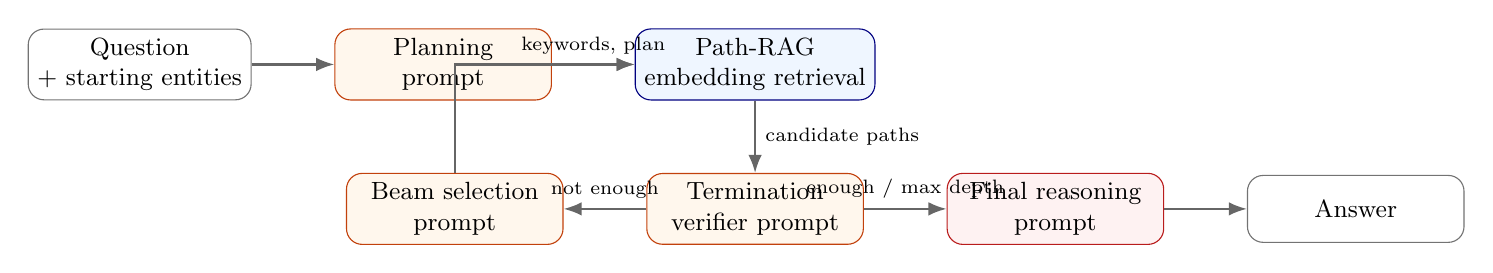
\begin{tikzpicture}[
  node distance=0.92cm and 1.05cm,
  box/.style={rectangle, rounded corners=2mm, draw=black!55, fill=white, align=center, minimum height=0.85cm, minimum width=2.75cm, font=\small},
  llm/.style={box, fill=softorange, draw=riskorange},
  risk/.style={box, fill=softred, draw=riskred},
  nonllm/.style={box, fill=softblue, draw=blue!50!black},
  arrow/.style={-{Latex[length=2.3mm]}, thick, draw=black!60}
]
\node[box] (q) {Question\\+ starting entities};
\node[llm, right=of q] (plan) {Planning\\prompt};
\node[nonllm, right=of plan] (rag) {Path-RAG\\embedding retrieval};
\node[llm, below=of rag] (verify) {Termination\\verifier prompt};
\node[llm, left=of verify] (beam) {Beam selection\\prompt};
\node[risk, right=of verify] (answer) {Final reasoning\\prompt};
\node[box, right=of answer] (out) {Answer};

\draw[arrow] (q) -- (plan);
\draw[arrow] (plan) -- node[above, font=\scriptsize]{keywords, plan} (rag);
\draw[arrow] (rag) -- node[right, font=\scriptsize]{candidate paths} (verify);
\draw[arrow] (verify) -- node[above, font=\scriptsize]{not enough} (beam);
\draw[arrow] (beam) |- (rag);
\draw[arrow] (verify) -- node[above, font=\scriptsize]{enough / max depth} (answer);
\draw[arrow] (answer) -- (out);
\end{tikzpicture}
}
\end{center}

\section*{Runtime Message Assembly}

Every chat prompt is assembled in \texttt{src/utils/llm\_backbone.py} as:

\begin{promptbox}{Message format}
\small
\texttt{[system prompt]} $\rightarrow$ \texttt{[few-shot examples]} $\rightarrow$ \texttt{[user prompt template]}.
The current generation parameters are \texttt{temperature=0}, \texttt{top\_p=0}, and \texttt{logprobs=False}.
\end{promptbox}

\section*{Prompt Inventory}

\begin{table}[h]
\centering
\small
\begin{tabular}{p{0.24\linewidth}p{0.22\linewidth}p{0.32\linewidth}p{0.11\linewidth}}
\toprule
Pipeline stage & Prompt object & Role in pipeline & Risk \\
\midrule
Planning / keyword generation & \texttt{plan\_prompt} & Produces keywords, planning steps, and declarative statement. & Medium \\
Path-RAG retrieval & No chat prompt & Embeds LLM-generated keywords and ranks KG relations/neighbors. & Medium \\
Path verbalization & \shortstack[l]{\texttt{reasoning\_path}\\\texttt{\_parser\_prompt}} & Converts symbolic KG path into natural language. & Medium \\
Termination verifier & \shortstack[l]{\texttt{terminals\_prune}\\\texttt{\_single\_prompt} or\\\texttt{deductive\_verifier}\\\texttt{\_prompt}} & Decides whether a path is sufficient or deductively supports a statement. & High \\
Beam candidate selection & \texttt{beam\_search\_prompt} & Chooses top candidate path indices. & Medium \\
Final answer & \texttt{reasoning\_prompt} & Produces the final answer from selected paths. & Critical \\
\bottomrule
\end{tabular}
\end{table}

\section*{Dataset Prompt Modules}

\begin{table}[h]
\centering
\small
\begin{tabular}{llll}
\toprule
Dataset flag & Prompt module & Final-answer risk phrase & Risk \\
\midrule
\texttt{RoG-webqsp} & \texttt{src/prompts/webqsp.py} & \texttt{and your knowledge} & Critical \\
\texttt{RoG-cwq} & \texttt{src/prompts/cwq.py} & \texttt{and your knowledge} & Critical \\
\texttt{CL-LT-KGQA} & \texttt{src/prompts/cl\_lt\_kgqa.py} & \texttt{and your knowledge} & Critical \\
\bottomrule
\end{tabular}
\end{table}

\section*{Faithfulness Risk Points}

\begin{itemize}[leftmargin=1.4em, itemsep=0.35em]
  \item \textbf{Final answer can use pretrained knowledge.}
  The prompt explicitly permits parametric knowledge, so high accuracy does not prove KG-grounded reasoning.

  \item \textbf{CR-LT True/False is vulnerable to random guessing and prior knowledge.}
  A binary task can achieve about 50\% by guessing, and the current prompt does not require KG-only entailment.

  \item \textbf{The verifier is LLM-mediated.}
  The verifier can judge path sufficiency using outside knowledge unless the prompt forbids it.

  \item \textbf{Path verbalization can add information.}
  The parser may transform a sparse symbolic path into a stronger natural-language claim than the KG path directly supports.
\end{itemize}

\section*{Representative Prompt Snippets}

\begin{promptbox}{Final answer prompt, WebQSP/CWQ}
\small
Given a question and the associated retrieved reasoning path from a knowledge graph, you are asked to answer the following question based on the reasoning path and your knowledge.\\
\texttt{Question: \{question\}}\\
\texttt{Reasoning path: \{reasoning\_path\}}\\
Only return the answer to the question.
\end{promptbox}

\begin{promptbox}{Final answer prompt, CR-LT}
\small
The CR-LT system message asks for True or False, but the final user prompt still uses the same wording:
\emph{based on the reasoning path and your knowledge}.
\end{promptbox}

\begin{promptbox}{Deductive verifier prompt}
\small
Whether the conclusion \texttt{\{declarative\_statement\}} can be deduced from \texttt{\{parsed\_reasoning\_path\}}, if yes, return yes, if no, return no.
\end{promptbox}

\section*{Pointers}

The full prompt dump with all examples is available in:
\begin{itemize}[leftmargin=1.4em]
  \item \texttt{docs/fidelis\_pipeline\_prompts.md}
  \item \texttt{docs/fidelis\_pipeline\_prompts.txt}
\end{itemize}

\end{document}
